% ======================================================================
% SECTION 07: RESULTS EVIDENCE AND VALIDATION
% ======================================================================
\section{Results Evidence and Validation}

We validated the upgraded Bronze/Silver modules and the new Gold pipeline across three checks: running all three DAGs inside the custom OpenJDK~17 Airflow container, inspecting both generated Gold Parquet summaries, and running the automated test suite.

\subsection{Gold Governance and Storytelling Parquet Results}
Executing the Gold Airflow DAG inside Docker produced two compact, verified Gold Parquet datasets: a governance summary (113 KPI rows, $6.57\text{ KB}$) and a storytelling summary (84 aggregation rows, $9.49\text{ KB}$). Table~\ref{tab:gold_results} presents representative records read directly from both files, and Fig.~\ref{fig:gold_storytelling} visualizes the resulting storytelling indicators.

\begin{table*}[!t]
\centering
\caption{Selected Verified Outputs Read from Both Gold Parquet Datasets (Governance: 113 Rows; Storytelling: 84 Rows)}
\label{tab:gold_results}
\scriptsize
\renewcommand{\arraystretch}{1.05}
\begin{tabularx}{\textwidth}{p{2.0cm} p{2.9cm} r r r l X}
\toprule
\textbf{Gold Dataset} & \textbf{Metric / Dimension} & \textbf{Primary} & \textbf{Secondary} & \textbf{Extra} & \textbf{Status / Tier} & \textbf{Interpretation} \\
\midrule
\textbf{Governance} & Silver Rows Read & 4,786 & 7 files & --- & PASS & Multi-run folder scan across Silver partitions. \\
\textbf{Governance} & Unique Events & 3,806 & 20.48\% dup & --- & PASS & 980 overlapping snapshot rows removed cleanly. \\
\textbf{Governance} & Schema Compliance & 100.00\% & 3,806 valid & 3 rej. & PASS & All Silver rows satisfy coordinate and magnitude bounds. \\
\textbf{Governance} & Pinned 10 km Depth & 31.69\% & 1,206 events & --- & WARN & Teleseismic fixed-depth artifact flagged above 25\%. \\
\textbf{Governance} & Depth IQR Outliers & 16.92\% & 644 events & $Q_2=10$ & WARN & Intermediate and deep subduction events preserved. \\
\textbf{Governance} & Linear Energy Outliers & 15.74\% & 599 events & 0\% log & WARN & Confirms why logarithmic energy is used for SAAI. \\
\textbf{Governance} & Cross-Source Pairs & 568 & 91.9\% match & --- & PASS & High historical reconciliation between USGS and EMSC. \\
\midrule
\textbf{Storytelling} & Minor ($M < 3.0$) & 2,058 & 54.07\% & $\mu_M=1.61$ & INFO & Dominant volume from local networks; minimal energy. \\
\textbf{Storytelling} & Moderate ($4.5\text{--}5.4$) & 1,347 & 35.39\% & $\mu_M=4.78$ & INFO & Core global seismicity across USGS and EMSC. \\
\textbf{Storytelling} & Strong \& Major ($\ge 5.5$) & 91 & 2.39\% & $M_{\max}=6.80$ & INFO & Rare events releasing $>99.8\%$ of seismic energy. \\
\textbf{Storytelling} & Peak SAAI (2026-11-16) & $\text{SAAI}=1.52$ & 228 events & $M_{\max}=6.60$ & ELEVATED & Strongest combined frequency and energy anomaly day. \\
\textbf{Storytelling} & Peak SAAI (2026-11-21) & $\text{SAAI}=1.03$ & 54 events & $M_{\max}=6.80$ & ELEVATED & Major $M\,6.8$ rupture elevating daily energy score. \\
\textbf{Storytelling} & Top Region (Milford, UT) & 125 & 3.28\% & $M_{\max}=3.12$ & NORMAL & High-frequency local swarm in Utah. \\
\textbf{Storytelling} & Top Subduction (Mindanao) & 51 & 1.34\% & $M_{\max}=5.90$ & ELEVATED & Active Philippine subduction zone sequence. \\
\textbf{Storytelling} & Shallow Depth ($0\text{--}70\text{ km}$) & 3,376 & 88.70\% & $\mu_Z=12.8\text{ km}$ & INFO & Highest surface shaking and tsunami hazard regime. \\
\bottomrule
\end{tabularx}
\end{table*}

\begin{figure*}[!t]
\centering
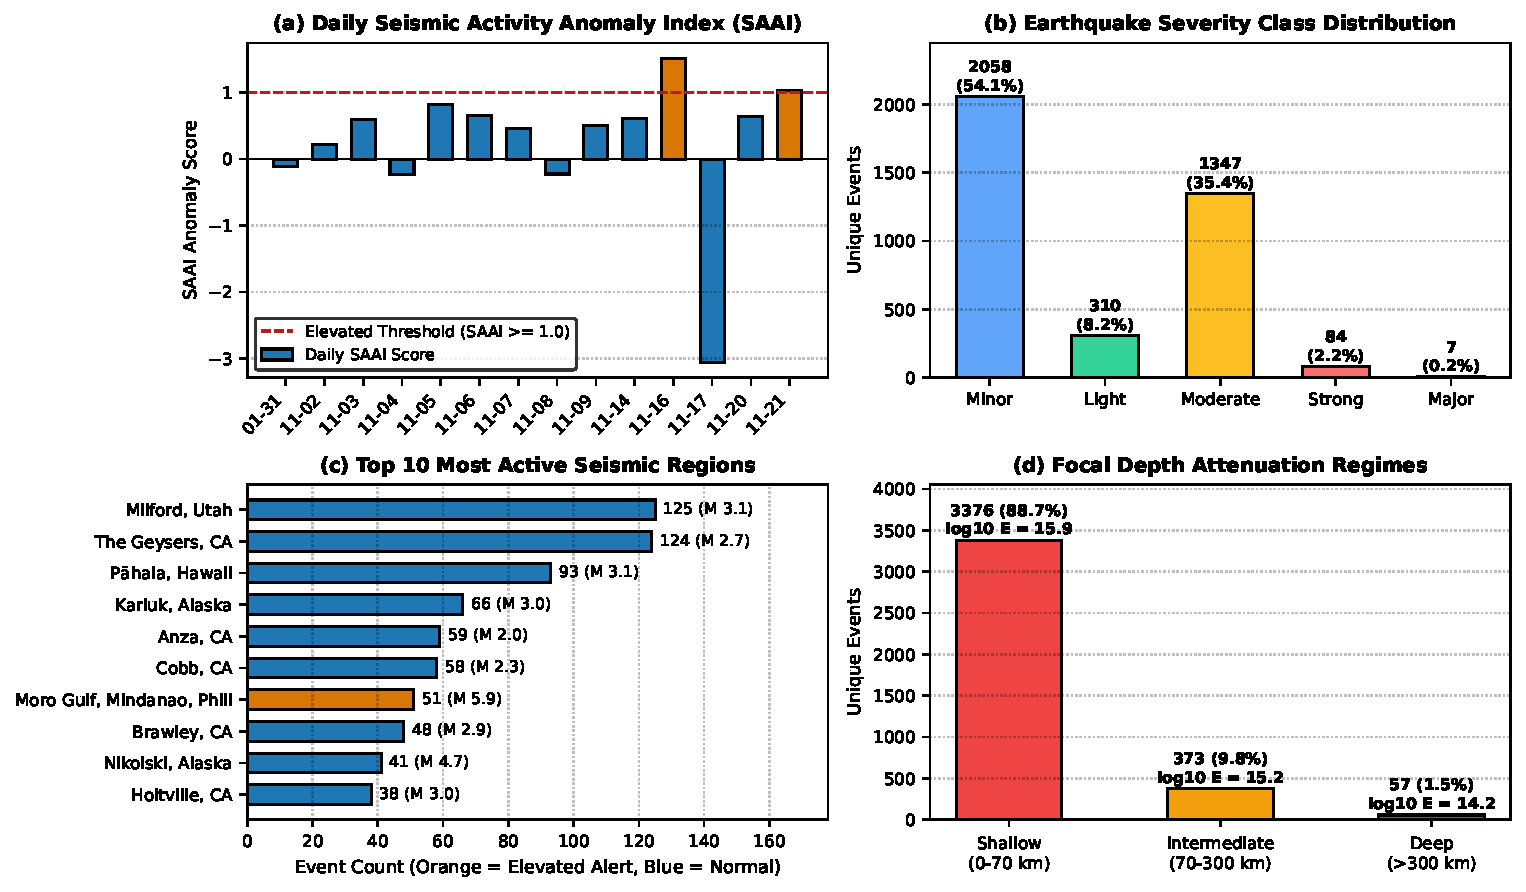
\includegraphics[width=0.90\textwidth]{figures/fig2_gold_storytelling_saai.pdf}
\caption{Visual summary of the Gold storytelling Parquet dataset: (a)~daily SAAI anomaly trend highlighting 2026-11-16 and 2026-11-21 as Elevated; (b)~earthquake severity tier distribution; (c)~top 10 most active seismic regions by alert tier; and (d)~focal depth attenuation regimes.}
\label{fig:gold_storytelling}
\end{figure*}

\subsection{Database State, Idempotency, and Automated Tests}
Checking the live PostgreSQL status confirms that all seven canonical tables are active and synchronized (Table~\ref{tab:db_status}). Historical sample loads, live partitioned API queries (59 USGS and 228 EMSC records for November 2025), and incremental polls populated 3,305 canonical events across all four sources, quarantined 3 malformed real-time rows, saved watermarks for every feed, and linked 1,274 duplicate agency detections into 637 unified earthquake groups ($\text{median }\Delta t = 0.47\text{ s}$, $\text{median }\Delta d = 6.33\text{ km}$). Re-running historical ingestion inserted zero new rows, proving full idempotency.

\begin{table}[H]
\centering
\caption{Live Canonical PostgreSQL State Verified After Multi-Source Ingestion}
\label{tab:db_status}
\renewcommand{\arraystretch}{1.12}
\resizebox{\columnwidth}{!}{%
\begin{tabular}{l r l}
\toprule
\textbf{Canonical Table} & \textbf{Rows} & \textbf{Verification Role} \\
\midrule
Sources & 4 & USGS Hist, EMSC Hist, USGS RT, GDACS RT \\
Events \& Earthquakes & 3,305 & 1,761 USGS RT, 855 EMSC, 677 USGS Hist, 12 GDACS \\
Event Groups & 1,274 & 637 unified multi-source earthquake groups \\
Quarantined Records & 3 & Missing-magnitude USGS RT rows stored as JSONB \\
Ingestion Runs & 10 & All 10 runs succeeded; re-runs inserted 0 duplicates \\
Watermarks & 4 & Active high-water mark stored for every feed \\
\bottomrule
\end{tabular}%
}
\end{table}

Finally, the automated test suite passes all 12 unit and integration tests (100\% pass rate in $1.1\text{ s}$), covering multi-format parsing, quarantine rejection reasons, Haversine distance accuracy, collision-free nearest-neighbor and three-way transitive grouping, 24-hour watermark overlap filtering, database schema constraints, and Gold Parquet schemas. Both Gold datasets are verified and ready to power the interactive dashboards in Workshop~\#4.
